\begin{frame}{$d(K^-, n)"\pi^-\Sigma^+"$と$d(K^-, n)" \pi^+\Sigma^-"$の平均 (\textcolor{red}{\bf Revised})}
  \label{page:ave_CS}
  
  \centering  
  \scriptsize
  %% 前のページの$d(K^-, n)"\pi^{\mp}\Sigma^{\pm}"$の平均。\\
  %% エラーはフィッティングエラーは各荷電モードの自乗平均で計算。\\
  %% 統計エラーとスケールファクターエラーは計算後に共通につける。\\

  \begin{figure}
    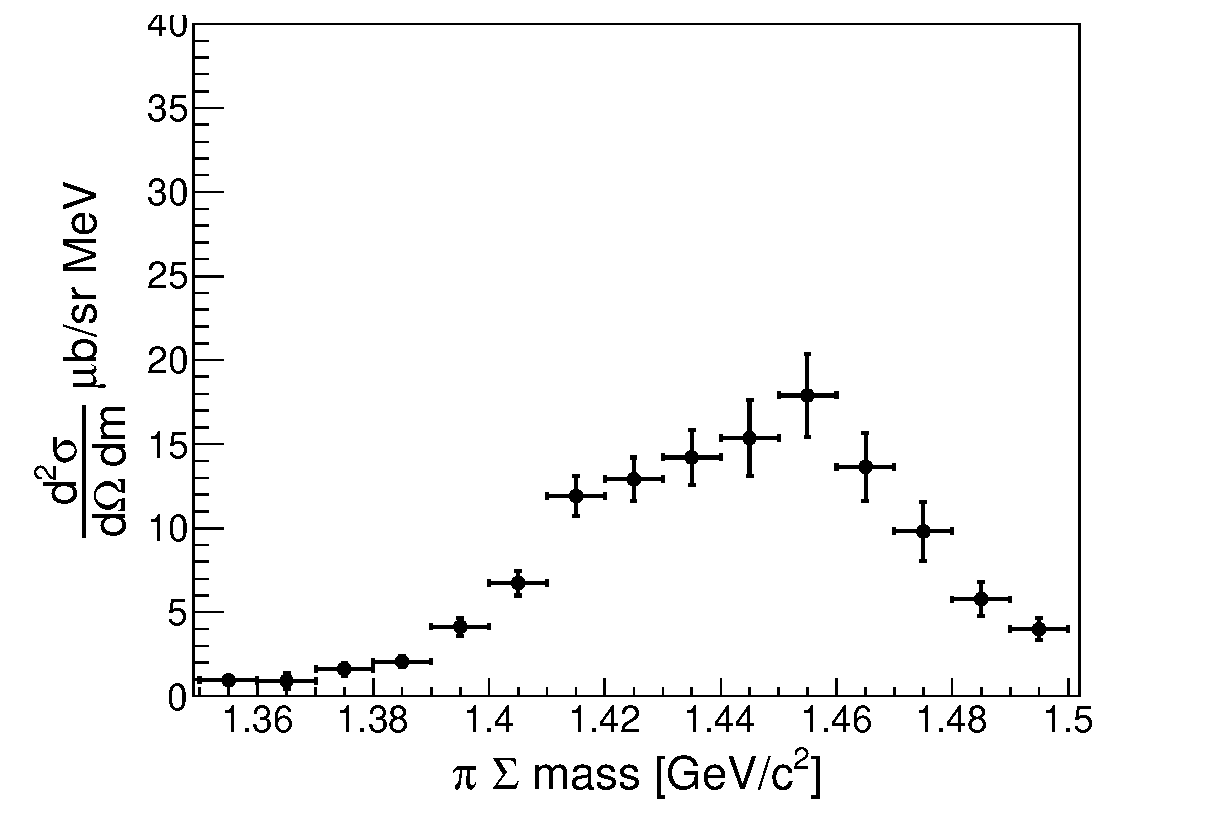
\includegraphics[width=6cm]{../pic/Run78//KN_ana_NC170_2sigma//Charge_ave_CS.eps}
  \end{figure}

  \begin{itemize}
  \item 内側Boxのエラー
    $ Err_{stat}=\frac{d\sigma_{ave}}{dM d\Omega}\times\frac{1}{\sqrt{N}} $ N : $d(K^-, n)"\pi^{\mp}\Sigma^{\pm}"$の各ビンのイベント数
  \item 外側Boxのエラー
    $
    Err_{stat+Fit}=\sqrt{\left(\frac{d^2\sigma_{ave}}{dM d\Omega}\right)^2\frac{1}{N}+
      \left(0.5Err_{\pi^+\Sigma^-}\right)^2+\left(0.5Err_{\pi^+\Sigma^+}\right)^2 }
    $
  \item エラーバー
    $
    Err_{stat+Fit+conv}=\sqrt{\left(\frac{d^2\sigma_{ave}}{dM d\Omega}\right)^2\frac{1}{N}+
      \left(0.5Err_{\pi^+\Sigma^-}\right)^2+\left(0.5Err_{\pi^+\Sigma^+}\right)^2+
      \left(\frac{d^2\sigma_{ave}}{dM d\Omega}Err_{conv}\right)^2 }
    $    
  \end{itemize}
    
  
  %% 内側のBoxは統計エラーを外側のBoxはフィッティングエラーを含むエラーを、\\
  %% エラーバーはスケールファクター[左表]を含むエラーを表す。\\
  %% 各エラーは自乗平均で計算。\\
\end{frame}
